\chapter{Теоретические исследования}
\label{chapter2}

В данной главе будут представлены основные результаты работы. Сначала будет рассмотрен основные кандидаты для гибридизации. Затем будет представлен анализ работы кандидатов на разных входных данных. Потом будет сделано некоторое предположение на основании экспериментов и на его основе сформулирован алгоритм гибридизации. 

\section{Основные кандидаты для гибридизации}

\subsection{Алгоритм на основе метода разделяй и властвуй}

Далее в работе этот алгоритм, для краткости, будет называться Fast.

Основная идея данного алгоритма аналогична идее алгоритма сортировки массива QuickSort. Множество точек разделяется медианой, и все точки разделяются на три множества: меньшие, равные и большие медианы по какому-либо критерию, причем можно сразу сказать, что точки первого множества доминируют над точками второго, которые в свою очередь доминируют над точками третьего. Далее алгоритм запускается рекурсивно на этих множествах.

%Опишем данный алгоритм более детально. 
%Пусть $q_k$ - это $k$-ый критерий функции приспособленности $q$, $q_{1:k}$ - это первые $k$ критериев. Выражение $q_{1:k} \prec t_{1:k}$ означает, что $q$ доминирует $t$ по первым $k$ критериям. Обозначим $RANK(q)$ - ранг функции приспособленность $q$.
Для понимания сути алгоритма Буздалова и др. \cite{Buzdalov} опишем основные моменты. Самый большой для нас интерес представляет процедура $NDHelperA$.

$NDHelperA$ принимает множество точек $S$ и номер рассматриваемого критерия $k$.  Далее, как написано выше, разделяем на 3 множества L, M, H, основываясь только на k критерии. L и H запускам рекурсивно, при этом продолжаем рассматривать k критерий. А M запускаем с номером критерием k-1.

Когда количество точек равно двум или количество критериев, по которым мы выявляем ранг, равно 2, рекурсивный запуск не происходит. Вместо этого запускается алгоритм сканирующей прямой, который подробно описан еще в статье Фортина \cite{Forton}. 

Таким образом по завершению процесса все точки проранжированы.   

%\begin{figure}[h]
%\begin{center}
%    \begin{algorithmic}[1]
%        \If {$|S|<2$}
%            \State {return}
%        \ElsIf {$|S|=2$}
%        	\State {$\{s^{(1)}, s^{(2)}\} \gets S$}
%        	\If {$s^{(1)} \prec s^{(2)}$} 
%        	\State { 
%        	$RANK(s^{(2)}) \gets max\{RANK(s^{(2)}),RANK(s^{(1)})+1\}}$
%        	\EndIf
%        \ElsIf {$k = 2$}
%    \end{algorithmic}
%    \caption{Процедура $NDHelperA$, которая назначает ранги точкам из $S$ используя первые $k$ критериев.}
%    \label{pseudo}
%\end{center}
%\end{figure}

\subsection{Алгоритм Best Order Sort}
Далее в работе этот алгоритм, для краткости, будет называться BOS.

Данный алгоритм создает отсортированный списки точек соответствующие каждому критерию (см. \ref{bos_descr}). Если у точек критерии совпадают, используется порядок, основанный на предыдущих критериях. Далее просматриваем точки начиная с первых в этих списках, переходя от списка к списку, потом переходим ко вторым точкам в этих списках. Ранг назначаются точкам при первой встречи, если точка уже имеет ранг, она пропускается. 

\begin{figure}
\begin{center}
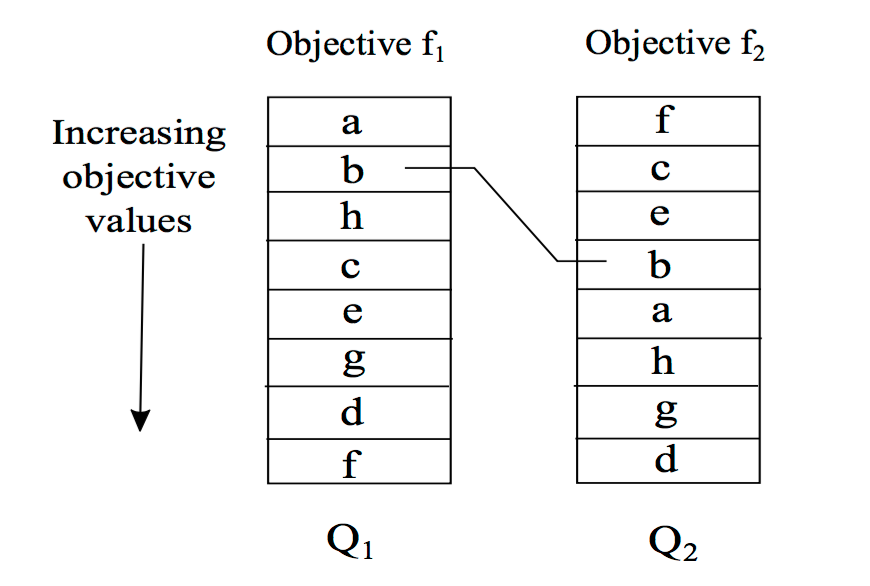
\includegraphics[width=8cm]{pic/bos_pic}
\caption{На рисунке представлены отсортированные списки по критерию f1 и f2. Точка b будет сравниваться только с точкой a и в последствии ее ранг не будет меняться.}
\label{bos_descr}
\end{center}
\end{figure}

Более детальное описание алгоритма не так существенно, так как алгоритм BOS встраивается в алгоритм Fast, и его внутреннее устройство не очень интересно. 

\section{Идеи гибридизации}
Простейший способ гибридизации двух вышеупомянутых алгоритмов -- создание алгоритма, который будет по входным данным выбирать один из двух алгоритмов и запускать его. Он должен принимать решение выбора алгоритма не медленнее, чем время работы выбранного им алгоритма.

Однако мы можем воспользоваться тем, что алгоритм Fast использует рекурсивный запуск себя же. В момент рекурсивного запуска мы можем запускать на подмножестве не тот же самый алгоритм, а алгоритм BOS. Причем в данном случае решение требуется принимать еще быстрее, так как оно принимается неоднократно.

Следовательно, наша основная задача заключается в том, чтобы быстро на каждом этапе выбирать наилучший алгоритм.  


\section{Анализ работы кандидатов}

Эти два алгоритма были выбраны в качестве основных кандидатов на гибридизацию именно из-за их асимптотики. Как указано в \cite{Buzdalov}, алгоритм Fast работает за $O(N\log^{M - 1}N)$. Алгоритм BOS работает в лучшем случае за $\Theta(MN\log{M})$, а в худшем случае -- за $\Theta(MN^2)$ \cite{BOS}. Можно видеть, что лучший и худший случаи у алгоритма BOS очень разнятся: при фиксированном числе критериев  $M$ BOS работает в лучшем для себя случае асимптотически лучше, чем Fast, однако он проигрывает, если попадает в худший для себя случай.

\section{Гибридный алгоритм}

В данной секции я опишу свой гибридный алгоритм, когда соберу больше данных по работе кандидатов